%\documentclass[aps,prd,preprint,showpacs,superscriptaddress,amsmath]{revtex4}
\documentclass[prd,showpacs,superscriptaddress,twocolumn,
floatfix,preprintnumbers,altaffilletter]{revtex4}

\usepackage{longtable}
\usepackage{graphicx}
\usepackage{amsmath,amssymb}
\usepackage{color}
\usepackage{units}
\usepackage{epstopdf}
\usepackage{hyperref}
\usepackage{multirow}
\newcommand{\braket}[2]{\left\langle#1\, |\,#2\,\right\rangle}  %  < #1 | #2 >
\newcommand{\expec}[1]{\langle#1\rangle}  %  < #1 >
\newcommand{\drm}{{\rm d}}
\newcommand{\irm}{{\rm i}}
\newcommand{\beq}{\begin{equation}}
\newcommand{\eeq}{\end{equation}}
\newcommand{\bdm}{\begin{displaymath}}
\newcommand{\edm}{\end{displaymath}}
\newcommand{\T}[1]{\tilde{#1}}
\newcommand{\wT}[1]{\widetilde{#1}}
\newcommand{\Cdot}{\!\cdot\!}
\newcommand{\SNR}{\textnormal{SNR}}
\newcommand{\rednote}[1]{{\color{red} (#1)}}
\definecolor{Gray}{gray}{0.9}

\graphicspath{{./plots/}}
\begin{document}

\pacs{95.75.-z,04.30.-w}

\title{The missing component: maximizing the sensitivity of post-merger gravitational-wave searches using principal component analysis}
\author{M Coughlin}
\affiliation{Division of Physics, Math, and Astronomy, California Institute of Technology, Pasadena, CA 91125, USA}
\email{mcoughli@caltech.edu}
\author{S Coughlin}
\email{scottcoughlin2014@u.northwestern.edu}
\affiliation{Physics and Astronomy, Cardiff University, Cardiff, CF10 2FH, UK}
\affiliation{Center for Interdisciplinary Exploration \& Research in 
(CIERA), Northwestern University, Evanston, IL 60208, USA}
\author{J Clark}
\affiliation{Department of Physics, Georgia Institute of Technology, Atlanta, GA 30332, USA}
\date{\today}

\begin{abstract}
  The detection of the post-merger signal from gravitational-wave compact binary coalescences by ground-based interferometric gravitational-wave detectors is an important goal for the advanced detector era.
  Searches of this signal type, where matched filtering is not possible, are commonly cast as pattern recognition problems, where the goal is to identify statistically significant clusters  indicating the presence of gravitational-wave transients in spectrograms of detector strain power when the precise signal morphology is unknown.
  Traditionally, generic clustering algorithms are used to identify the clusters.
  In this study, we explore the use of principal component analysis based template banks for the use in clustering.
  We show that the use of these template banks can significantly improve the sensititivity of searches for signals with these morphologies.
\end{abstract}

\maketitle

The detection of unmodeled gravitational-wave transients by ground-based interferometric gravitational-wave detectors such as Advanced LIGO~\cite{aligo} and Advanced Virgo~\cite{avirgo} is an important goal for the advanced detector era.
Detections of this type will complement the recent detections of gravitational waves from binary black holes \cite{AbEA2016a,AbEA2016e,AbEA2017a,AbEA2017c} and binary neutron stars \cite{AbEA2017b}.
There is a spectrum to the knowledge of sources that these detectors will be targeting.
On one end are searches for compact binaries, such as binary neutron stars (BNSs), neutron-star black holes (NSBHs), and binary black holes (BBHs), which are well-modeled and therefore use matched filtering to perform searches \cite{AaEA2013b,AbEA2012,AbEA2010}.
On the other end are searches for poorly modeled transients, such as long-lived narrowband GW transients proposed to originate in a variety of astrophysical processes, most notably, in newborn neutron stars~\cite{PiTh2012,Piro2011,Piro2007,CoMe2009} and black hole accretion disks following stellar collapse~\cite{KiSh2011,VaPu2001,VaPu2008}, that use minimal assumptions.

There is a middle-ground of sources, such as the GW emission by newly born magnetars \cite{StDa2005,SiRo2007,DaSh2009,GiPe2013,DaGi2015} or core-collapse supernovae \cite{Ott2009} for which numerical relativity simulations and waveform catalogs exist. 
Traditionally, waveform catalogs based on these waveforms have been used to perform parameter estimation and model selection of the signals of interest.
For the supernovae case in particular, there is a significant breadth of literature. 
Catalogs exist for various core-collapse mechanisms, including the neutrino mechanism \cite{Jan2012}, the magnetorotational mechanism \cite{BuDe2007}, and the acoustic mechanism \cite{BuLi2006}. 
Logue et al. \cite{LoOt2012} recently used PCA and a Bayesian formulism to perform model selection for these mechanisms.
Summerscales et al. \cite{SuBu2008} used the waveforms of Ott et al. \cite{OtBu2004} to perform parameter estimation and signal reconstruction.
Brady and Ray-Majumder \cite{BrRa2004} proposed using a Gram-Schmidt orthonormalization of supernovae waveform catalogs to inform gravitational-wave searches.
Heng \cite{Sio2009} used Principal Component Analysis (PCA) on the Dimmelmeier \cite{DiOt2008} waveform catalog and showed few components are required to represent the waveforms with matches above 0.9.
Cannon et al. \cite{CaCh2010} have also used this method for GW signals from compact binary coalescence.
Rover et al. \cite{RoBi2009} used PCA combined with Bayesian inference to perform signal reconstruction and parameter estimation.
PCA takes the set of waveforms (or any correlated, multi-dimensional data set) and returns a set of orthogonal components using the eigenvectors and eigenvalues of the covariance matrix of the data set.

While the above analyses used the waveform catalogs to perform parameter estimation and model selection, in general, they assume that a gravitational wave has been detected by a generic analysis.
We can take inspiration from this work to improve how searches are performed.
Most searches for unmodeled transients use seed-based nearest neighbor clustering of strain power spectrograms ~\cite{ThCo2013}, which identify GW signals by searching for pixels of excess power above some threshold, {\em seeds}, which leads to the creation of seeds along a spectrogram track.
The algorithm then uses a rule to connect neighboring seeds to form a cluster.
Detection statistics are then computed based on these clusters, which determine whether it is consistent with signal or noise.
These algorithms are beneficial for signal morphologies that have no or few defining characteristics.
After the recent detection of GW170817 and the search for a post-merger \cite{AbEA2017h}, there is significant interest in improved methodology for performing the searches, as well as more and more numerical relativity simulations available to inform searches.

In the case where more is known or assumed about a signal, other clustering strategies are possible. ``Seedless clustering,'' for example, uses the assumption that most models for long-duration gravitational-wave transients are narrow-band and therefore can be parameterized by narrow-band tracks in $ft$-maps \cite{ThCo2013,ThCo2014,CoTh2014,CoMe2015,CoMe2015b,ThCo2015}.
This algorithm integrates the signal power along spectrogram tracks using pre-defined ``templates'' chosen to capture the salient features of a wide class of signal models.
In this paper, we will combine the power of PCA catalogs and seedless clustering to search for gravitational-wave signals.
We will show that only a few PCA components are required to dramatically improve the results of the clustering and therefore the sensitivity to these particular signals.

\begin{figure*}[t]
 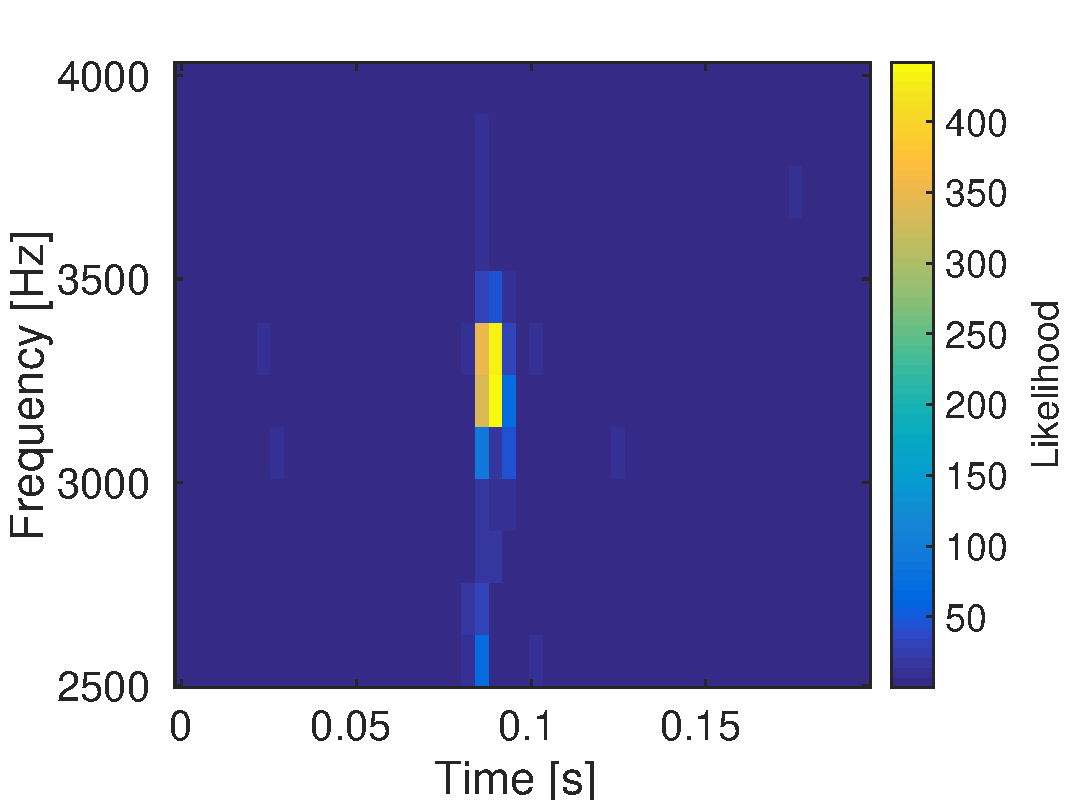
\includegraphics[width=3.5in]{map_PMNS.pdf}
 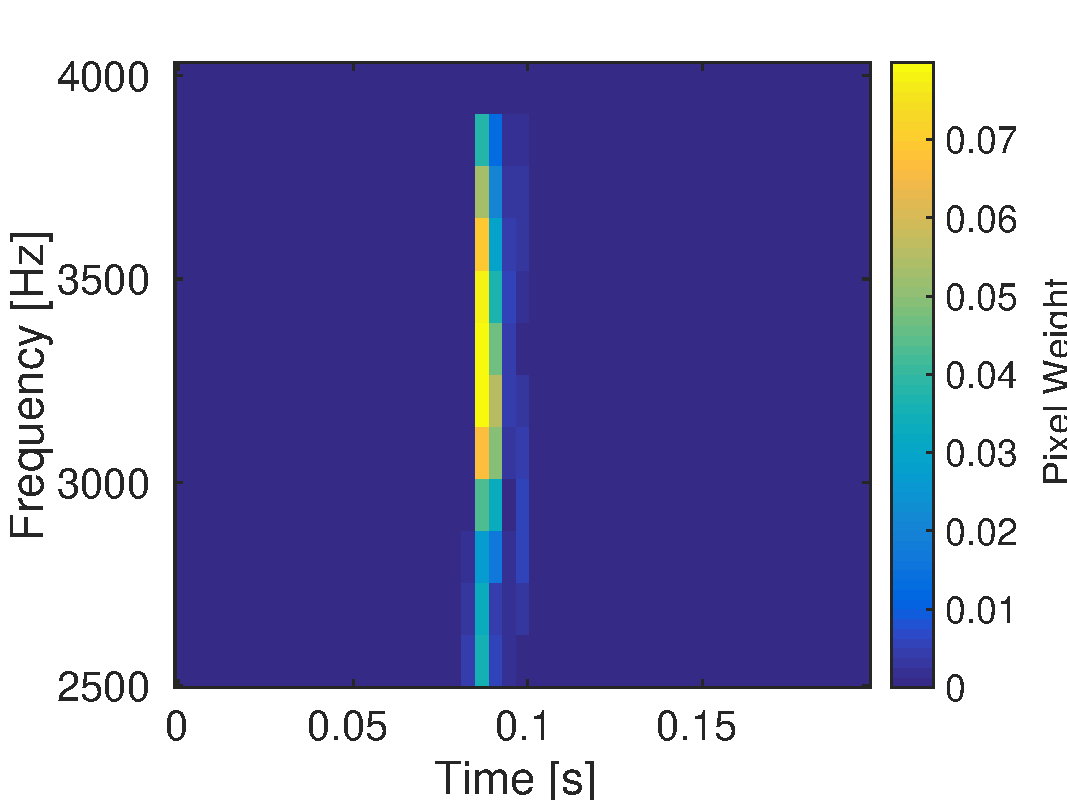
\includegraphics[width=3.5in]{rmap_H_PMNS.pdf} 
 %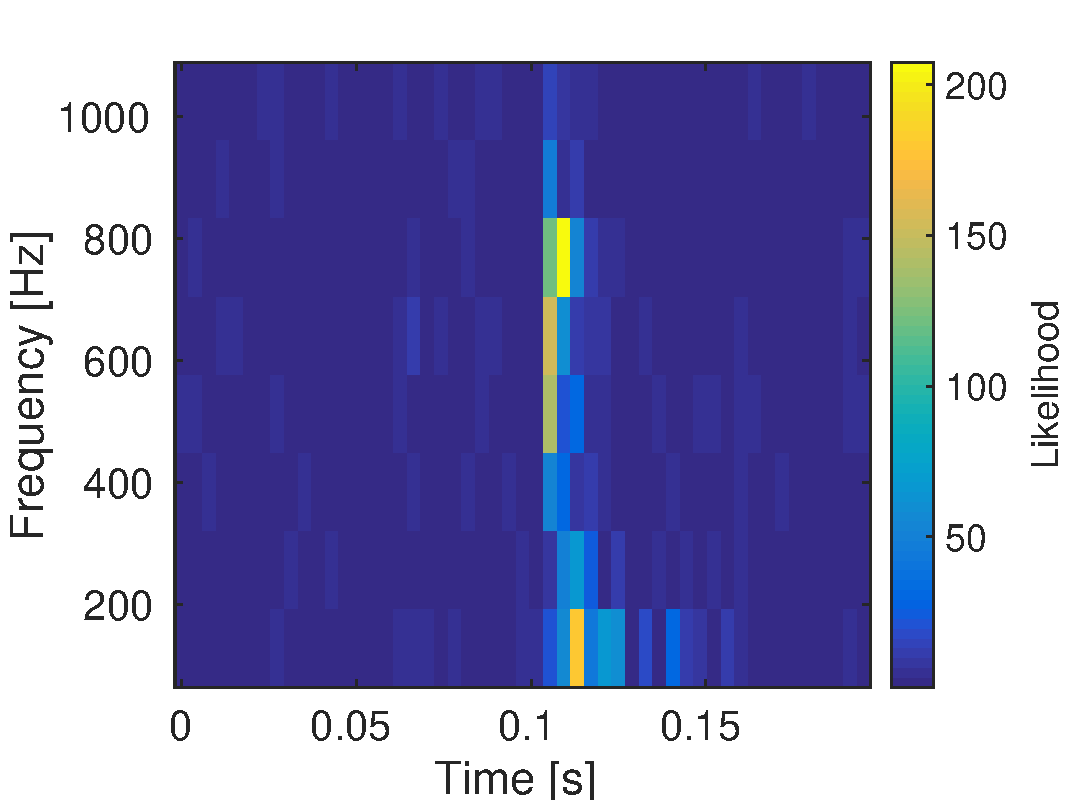
\includegraphics[width=3.5in]{map_DIM.pdf}
 %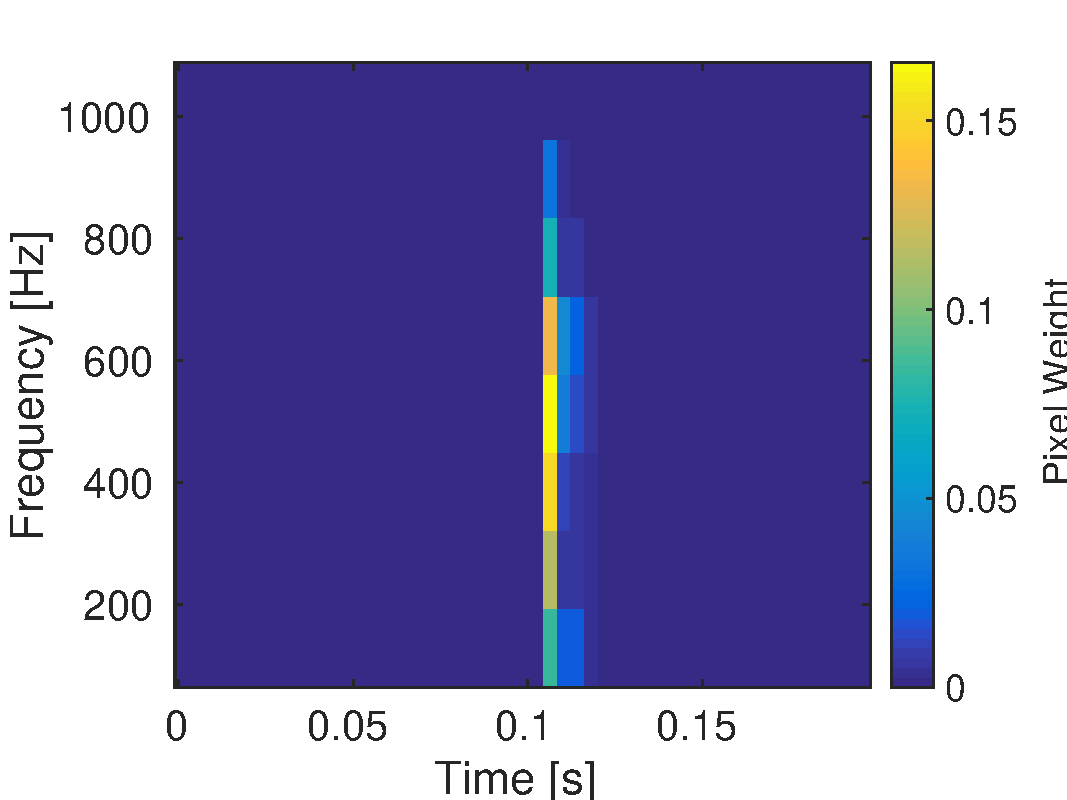
\includegraphics[width=3.5in]{rmap_H_DIM.pdf} 
 \caption{
   The plot on the left shows $\rho(t;f)$ for a simulated post-merger and supernova signal injected on top of Monte Carlo detector noise.
   The simulated noise is created for the advanced LIGO Hanford and Livingston Observatories operating at design sensitivity.
   The plot on the right shows the recovery obtained with seedless clustering for the injection.
 }
 \label{fig:SNR}
\end{figure*}

In the following, we briefly review how searches for unmodeled transients are typically performed.
Most searches for unmodeled GW transients use spectrograms proportional to GW strain power. 
Spectograms are created from pixels computed from dividing detector strain time series in segments and computing the Fourier transform of the segments. 
In the following, we denote the Fourier transform of strain data from detector $I$ for the segment with a mid-time of $t$ by $\tilde{s}_I(t;f)$. 
For the analysis below, we will use $50\%$-overlapping, Hann-windowed segments with duration of $\unit[0.0078125]{s}$ and a frequency resolution is $\unit[128]{Hz}$.
This segment duration is chosen to be of the order of the signal morphology time-scales.
Spectrograms are computed using a coherent detector statistic \cite{SuEA2010}. This statistic corresponds to the maximum amount of energy in the whitened data that is consistent with the hypothesis of a gravitational wave from a given sky position $\Omega$. 
\begin{equation}
\rho(t;f|\hat\Omega) = \vec{d(t;f)}^\dag (\vec{F} (\vec{F}^\dag \vec{F})^{-1} \vec{F}^\dag) \vec{d(t;f)}
\end{equation}
where $\vec{d}$ is the data in one whitened time-frequency pixel, $\vec{F} = (F^+, F^{\times})$ 
are the antenna factors, which in general depend on $t$, $f$, and $\hat\Omega$.

The problem at hand is to use the gravitational waveforms available from simulations to inform the clustering used in their detection.
Each waveform in the catalog corresponds to simulations with different initial conditions and simulation parameters, which in the supernovae case mean progenitor star mass or equation of state and for the neutron-star post-merger case mean binary mass and equation of state.
Because the exact waveform of the signal cannot be predicted in advance, one method is to use principal component analysis (PCA) on the waveform catalogs to analyze the gravitational-wave signals.
The principal components are computed using singular value decomposition on the waveforms in the catalog to create sets of orthogonal basis vectors, known as the Principal Components (PCs). These are placed in order from largest to smallest eigenvalue. The first eigenvector is therefore the most common feature of the waveforms in the catalog. Using the entire set of PCs, each waveform can be reconstructed exactly using the correct set of eigenvalues. By design, the original waveforms can be well-approximated by a small number of eigenvectors, which was originally shown by Heng \cite{Sio2009} and then Rover et al. \cite{RoBi2009}.

We now describe how the principal components are produced. Please see \cite{ClEA2015} for more details.
The PCs are obtained via singular value decomposition (SVD) of time-frequency map waveforms from each catalog. 
In the post-merger case, the waveforms are aligned by their peak in the post-merger spectrum generated by the dominant quadrupolar oscillation of the remnant.
The waveforms are placed in a matrix A (number of columns m corresponding to the number of waveforms in the catalog) with columns of equal length n.
To perform the SVD, A is recast as
\begin{equation}
A = U \Sigma V^T
\end{equation}
where $\Sigma$ is an $n \times m$ diagonal matrix whose entries are the square root of the eigenvalues of $A A^T$, U is an $n \times n$ matrix which columns equal to the eigenvectors of $A A^T$, and V is an $m \times m$ matrix whose columns are the eigenvectors of $A^T A$.
The principle components are then the eigenvectors of U and are ranked by their eigenvalues given in $\Sigma$.
The idea is that the original waveforms can be reconstructed by using a linear combination of the principle components, as
\begin{equation}
h_i = \sum_{j=1}^k U_j \beta_j.
\end{equation}
Here, $h_i$ is the reconstructed waveform from the catalog, $U_j$ is the jth principle component from the U matrix and $\beta_j$ is the corresponding principle component coefficient.
These components are computed by projecting $h_i$ onto $U_j$.
In general, the idea is to keep as many principle components, $k$, as desired for a given waveform accuracy.

We now describe the novel clustering algorithm applied in this search.
As described above, seedless clustering integrates pixels in $ft$-maps along parameterized tracks.
In searches for long-duration gravitational-wave transients, these have either been randomly generated B\'ezier curves~\cite{Far1996,ThCo2013,ThCo2014,CoMe2015b,ThCo2015}, a PN expansion for circular CBC signals \cite{CoTh2014}, and an analytic expression for low-to-moderate eccentric compact binaries \cite{CoMe2015} are all seedless clustering parameterizations previously used.
These parameterizations are used to create template banks of frequency-time tracks that are computed in parallel on multi-core devices such as graphical processor units (GPUs). 
In general, the total signal-to-noise ratio for a cluster of pixels can be written as a sum of over $\rho(t;f|\hat\Omega)$:
\begin{equation}\label{eq:sum}
  \text{SNR}_\text{tot} \equiv
  \frac{1}{N^{1/2}}
  \sum_{\left\{t;f\right\}\in\Gamma} \rho(t;f|\hat\Omega) ,
\end{equation}
The use of $ft$-maps as clustering parameterizations changes this implementation slightly. The PCA $ft$-maps provide not only the shape of the cluster in $ft$-map space but also amplitude information. 
Therefore we can rewrite the above algorithm as 
\begin{equation}\label{eq:sum}
  \text{SNR}_\text{tot} \equiv
  \sum_{\left\{t;f\right\}\in\Gamma} H(t;f) \rho(t;f|\hat\Omega) ,
\end{equation}
where $H(t;f)$ corresponds to the principal component cluster.

It will be necessary to randomize over coefficients in front of the principal component vectors of the catalog. 
In the case of the post-merger scenario, we will allow for two randomized variables in the seedless recovery. The first is simply the coefficient in front of the first principal component eigenvector. The second is particular to the post-merger scenario, which is known as $f_\textrm{peak}$, which is a peak in the post-merger spectrum generated by the dominant quadrupolar oscillation of the remnant, which is present in all models that form a neutron-star merger remnant. This frequency scales with the radii of non-rotating neutron stars. The PCA waveform catalogs are generated by aligning the main peaks of different catalog spectra to a common $f_\textrm{peak}$. The catalog is generated using a reference peak frequency of $f_\textrm{ref} = 2.6$\,kHz such that the factor for rescaling the frequency is $\frac{f_\textrm{ref}}{f_\textrm{peak}}$.
If we denote the mean time-frequency map as $M$, the time-frequency principal components as $U(t;f|f_\textrm{peak})_j$, the time-frequency principal component coefficients as $\beta_j$, the template $H(t;f)$ will take the form:
\begin{equation}
H(t;f) = M + U(t;f|f_\textrm{peak})_1 \beta_1
\end{equation}
where $H(t;f)$ is normalized to unity. In this case, $f_\textrm{peak}$ and $\beta_1$ are allowed to vary from $2500 - 4000$\,Hz and $-50 - 50$ respectively, which span the waveform catalogs.
In the case of the supernovae, we will sum over the first two time-frequency principal components, and therefore
\begin{equation}
H(t;f) = U(t;f)_1 \beta_1 + U(t;f)_2 \beta_2.
\end{equation}

\begin{figure*}[t]
 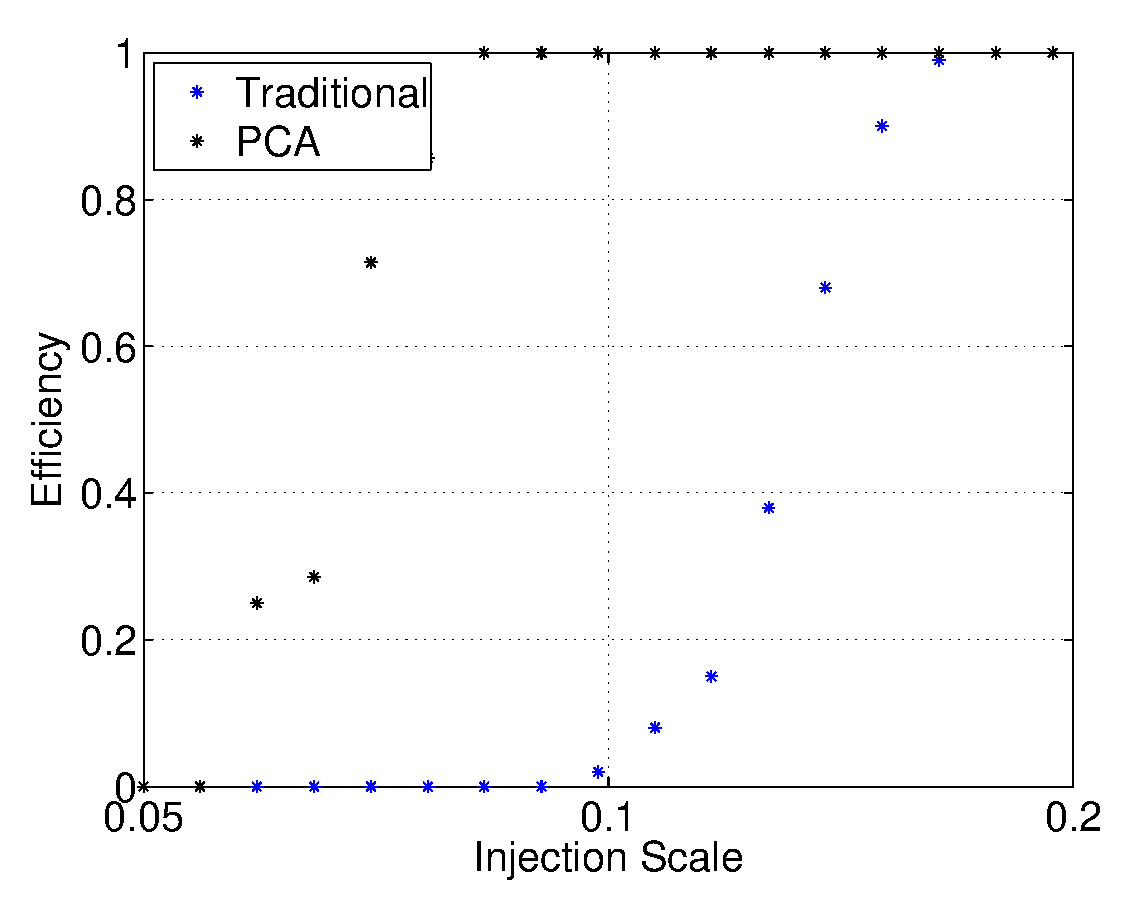
\includegraphics[width=3.5in]{X_seedless_eff.eps}
 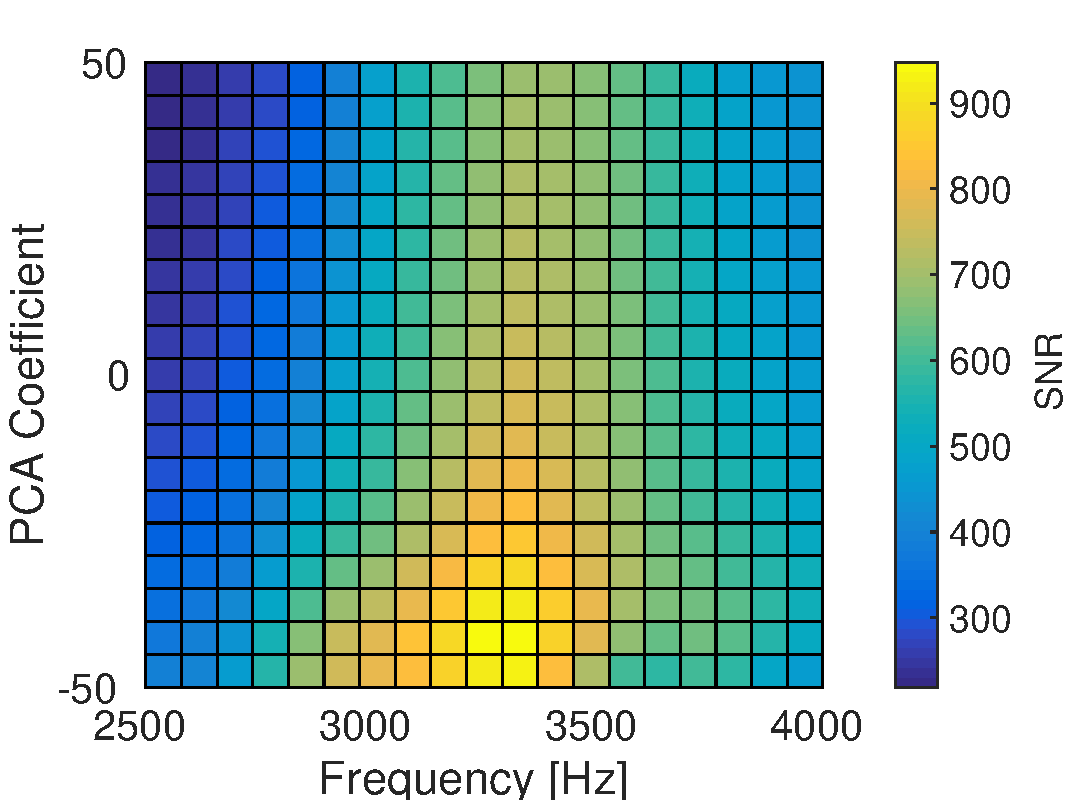
\includegraphics[width=3.5in]{paramest_PMNS.pdf}
 \caption{
   The left plot shows the efficiency curves using both the traditional nearest-neighbor clustering and PCA clustering for a simulated post-merger signal injected on top of Monte Carlo detector noise.
   The right plot shows the SNR recovered by the PCA components over different portions of the parameter space. The peak of the distribution is encompassed by the true values, which lie at $f_0 = 3254$ and $\beta = -31.5$.
 }
 \label{fig:results}
\end{figure*}

In this section, we describe a study to determine the potential increase in sensitivity of X-pipeline to the post-merger waveforms using simulated Monte Carlo noise.
We use a network of the Advanced LIGO detectors in Hanford, WA (H1) and Livingston, LA (L1)~\cite{aligo}.
Each waveform is injected into Monte Carlo Gaussian noise colored with the design sensitivity of Advanced LIGO.
The spectrograms are each $\unit[256]{s}$ in length, constructed with $50\%$-overlapping Hann windows. 
We use Hann-windowed segments with duration of $\unit[0.0078125]{s}$ and a frequency resolution of $\unit[128]{Hz}$.
Signals are injected at random sky locations $(\text{ra},\text{dec})$ (chosen from an isotropic distribution) and with random inclination and polarization angles $(\iota,\psi)$.
The left of figure~\ref{fig:results} shows the efficiency curves for the first waveform in the catalog. We compare the result from using both the traditional nearest-neighbor clustering and PCA clustering.
We compare the waveform amplitude to which the algorithms can detect a source with a false-alarm probability $\text{FAP}<0.1\%$ and a false-dismissal probability $\text{FDP}=50\%$.
The ratio of these amplitudes for the PCA and the traditional nearest-neighbor clustering is a factor of 2, indicating a potential increase in sensitive volume of a factor of 8.

We now explore the potential for parameter estimation using the above technique, for the purpose of potentially informing dedicated algorithms of the best fit at the clustering stage \cite{LoOt2012}. The right of figure~\ref{fig:results} shows the SNR recovered by the PCA components over different portions of the parameter space. The peak of the distribution is encompassed by the true values, which lie at $f_0 = 3254$ and $\beta = -31.5$. 

We have described an extension of current gravitational-wave clustering methods to account for waveform catalog knowledge using principal component analysis.
We showed how this algorithm can improve but signal reconstruction as well as signal-to-noise ratio improvements.
We find that this improvement comes at a modest computational cost.

There are a variety of avenues for research going forward.
For example, it could also be used to improve supernova searches with the waveform catalogs available.
In the future, we also intend to explore the possibility that this technique can be extended to a diverse waveform catalog.
This will allow for the determination of whether a single catalog (and therefore randomized coefficients) will be sufficient for gravitational-wave detection.
This is beneficial especially for models such as those considered above, where a variety of supernovae catalogs exist.

\acknowledgments
MC is supported by the David and Ellen Lee Postdoctoral Fellowship at the California Institute of Technology.
J. C. gratefully acknowledges support from NSF grants PHY-0955825, PHY-1212433, PHY-1333360, PHY-1505824 and PHY-1505524.
LIGO was constructed by the California Institute of Technology and Massachusetts Institute of Technology with funding from the National Science Foundation and operates under cooperative agreement PHY-0757058.

\bibliography{references}

\end{document} 
